\documentclass[xcolor=svgnames]{beamer}
\setbeamertemplate{caption}{\raggedright\insertcaption\par}
\usepackage[utf8]{inputenc}
\usepackage{xcolor}
\usepackage{booktabs, comment} 
\usepackage{csquotes}
\usepackage{amsmath}
\usepackage{tikz}
\usepackage{appendixnumberbeamer}
\usetheme{Madrid}
\usepackage[version=4]{mhchem}
\usepackage{adjustbox}
\usepackage{tikz}
\usepackage{tikzlings}
\usetikzlibrary{decorations.pathmorphing,arrows.meta}
\usepackage{cancel}
\usepackage{subcaption}
\usepackage{caption}
% redefines the caption setup of the figures environment in the beamer class.
\captionsetup[figure]{labelformat=empty}
\captionsetup[table]{labelformat=empty}

% COLORS 
\definecolor{mqred}{RGB}{166, 25, 46}
\definecolor{mqdeepred}{RGB}{118, 35, 47}
\definecolor{mqgray}{RGB}{55, 58, 54}
\definecolor{mqlightgray}{RGB}{237, 235, 229}
\definecolor{mqmagenta}{RGB}{198, 0, 126}
\usecolortheme[named=mqred]{structure}
\setbeamercolor{title in head/foot}{bg=mqlightgray, fg=mqgray}
\setbeamercolor{author in head/foot}{bg=mqdeepred}
\setbeamercolor{page number in head/foot}{bg=mqdeepred, fg=mqlightgray}
\usefonttheme[onlymath]{serif}

% FOOTNOTE ARRANGEMENTS

\makeatletter
\setbeamertemplate{footline}{
  \leavevmode%
  \hbox{%
  \begin{beamercolorbox}[wd=.5\paperwidth,ht=2.25ex,dp=1ex,center]{author in head/foot}%
    \usebeamerfont{author in head/foot}\insertshortauthor\expandafter\ifblank\expandafter{\beamer@shortinstitute}{}{~~(\insertshortinstitute)}
  \end{beamercolorbox}%
  \begin{beamercolorbox}[wd=.4\paperwidth,ht=2.25ex,dp=1ex,center]{title in head/foot}%
    \usebeamerfont{title in head/foot}\insertshorttitle
  \end{beamercolorbox}%
  \begin{beamercolorbox}[wd=.1\paperwidth,ht=2.25ex,dp=1ex,center]{page number in head/foot}%
    \usebeamerfont{page number in head/foot}\insertframenumber{} / \inserttotalframenumber 
  \end{beamercolorbox}}%
  \vskip0pt%
}
\makeatother
\beamertemplatenavigationsymbolsempty


% TITLE, AUTHORS, INSTITUTE, DATE

\title[Sympathetic Cooling Optimization]{Sympathetic Cooling Optimization for Precision Spectroscopy of Chiral Molecular Ions}
\author{Doron Behar}
\institute[Yuval Shagam's Group]{Technion Institute of Technology / Solid State Institute}
\date{\today}

% LOGO
\titlegraphic{
\includegraphics[width=0.8\linewidth]{graphics/logo.pdf}} % Change the logo path as needed

\begin{document}

\begin{frame}
    \titlepage
\end{frame}

\begin{frame}{Outline}
\tableofcontents
\end{frame}

\section{Simulation details \& Theoretical Background}

\begin{frame}{Simulating with LAMMPS}

\begin{figure}
    \centering
    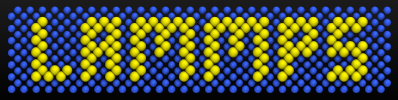
\includegraphics[width=0.5\linewidth]{graphics/lammps-logo.png}
    \caption{Many particles, classical motion propagation software package}
\end{figure}
Relevant Features:
\begin{itemize}
    \item[$+$] Can deal with $N(N-1)$ Coulomb interactions in $\mathcal{O}(1)$ complexity using GPU.
    \item Accepts analytical expressions of $\mathbf{E}(\mathbf{r}, t)$
    \item[$+$] Calculates ions' motions faster then writing results to disk
    \item[$+$] Has an excellent Python API
\end{itemize}
\end{frame}

\begin{frame}{Time Steps Considerations}
\begin{itemize}
    \item Simulation time scale is defined by RF period $T_\mathrm{rf}$.
    \item[$\Rightarrow$] Dividing $T_\mathrm{rf}$ to integer $t_d = \mathcal{O}(1500)$ time steps is desired.
    \item Convergence is checked by increasing $t_d$ and checking results are similar, with no 'Coulomb Force Explosion'.
\end{itemize}

\begin{columns}

\begin{column}{0.6\textwidth}
\begin{figure}
    \centering
    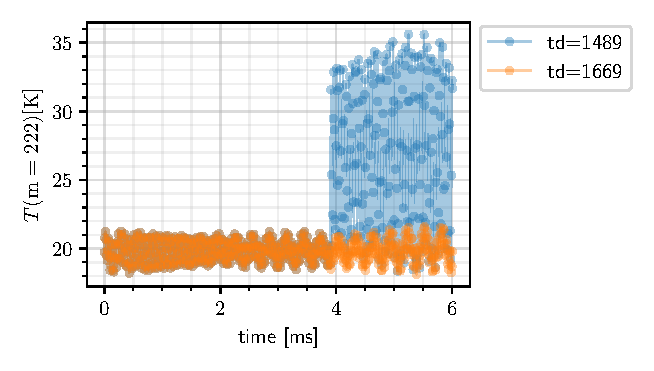
\includegraphics[width=\linewidth]{graphics/convergence-example.pdf}
\end{figure}
\end{column}

\begin{column}{0.4\textwidth}
\begin{figure}
    \centering
    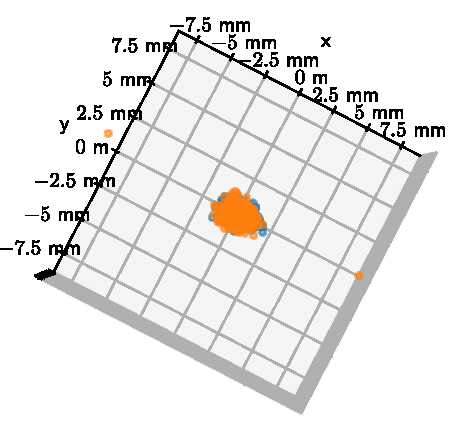
\includegraphics[width=\linewidth]{graphics/coulomb-explosion.pdf}
\end{figure}
\end{column}

\end{columns}
\end{frame}

\begin{frame}{Ion Trapping}{Analysis}
Problem: Laplace equation: $\nabla^2\phi = 0$
$$\text{Solution:}\ \phi = \sum_{i\in\{x,y,z\}} x_i^2 \left(a_i + q_i \cos(2\pi f_\mathrm{rf} t)\right),\ \sum_{i\in\{x,y,z\}} a_i = \sum_{i\in\{x,y,z\}} q_i = 0$$

\begin{columns}

\begin{column}{0.33\textwidth}
\begin{figure}
    \centering
    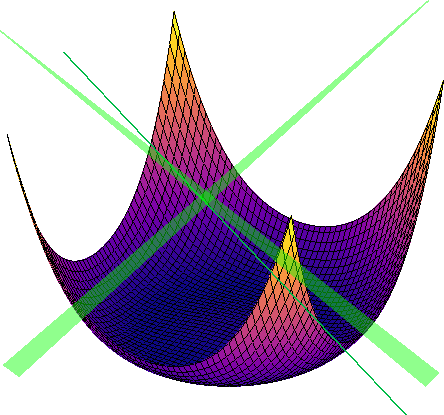
\includegraphics[width=\linewidth]{graphics/ion-trap-basics@effective.pdf}
\end{figure}
\end{column}

\begin{column}{0.33\textwidth}
\begin{figure}
    \centering
    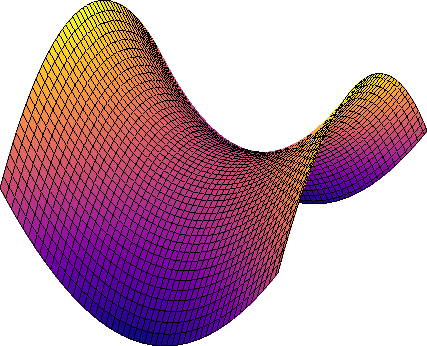
\includegraphics[width=\linewidth]{graphics/ion-trap-basics@0.pdf}
    \caption{$f_\mathrm{rf} t=0$}
\end{figure}
\end{column}

\begin{column}{0.33\textwidth}
\begin{figure}
    \centering
    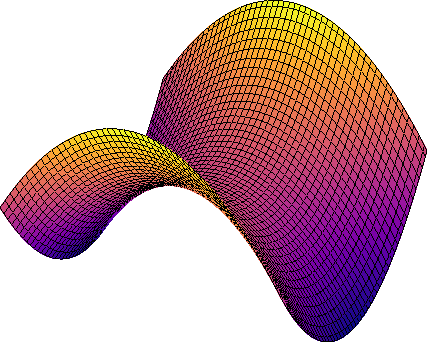
\includegraphics[width=\linewidth]{graphics/ion-trap-basics@Pi.pdf}
    \caption{$f_\mathrm{rf} t = 1/2$}
\end{figure}
\end{column}

\end{columns}

\end{frame}

\begin{frame}{1D Single Ion Trap: Mathieu Equation}

$$\phi = \sum_{i\in\{x,y,z\}} x_i^2 \left(a_i + q_i \cos(2\pi f_\mathrm{rf} t)\right) \Rightarrow \ddot{x}_i = \left(\tilde{a}_i + 2\tilde{q}_i\cos(2\tau)\right) x$$

\begin{figure}
    \centering
    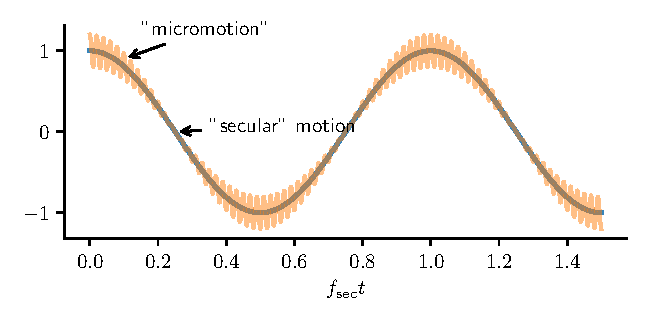
\includegraphics[width=0.8\linewidth]{graphics/micromotion-illustration.pdf}
    \caption{$f_\mathrm{sec}\underset{\text{typically}}{\ll} f_\mathrm{rf}$}
\end{figure}

\end{frame}

\begin{frame}{Mathieu Equation Solved Inversely}
\begin{columns}

\begin{column}{0.4\textwidth}
$$(\tilde{a}_i, \tilde{q}_i) \rightarrow f_\mathrm{sec}$$
$$\begin{pmatrix}
    \tilde{a}_x & \tilde{q}_x \\
    \tilde{a}_y & \tilde{q}_y \\
    \tilde{a}_z & \tilde{q}_z \\
\end{pmatrix} \mathcolor{red}{\overset{?}{\leftarrow}} \begin{pmatrix}
    f_\mathrm{sec(x)} \\
    f_\mathrm{sec(y)} \\
    f_\mathrm{sec(z)}
\end{pmatrix}$$
$$\begin{pmatrix}
    \sum_i \tilde{a}_i = 0 \\
    \sum_i \tilde{q}_i = 0 \\
    q_z= 0
\end{pmatrix}$$
\end{column}

\begin{column}{0.6\textwidth}
\begin{figure}
    \centering
    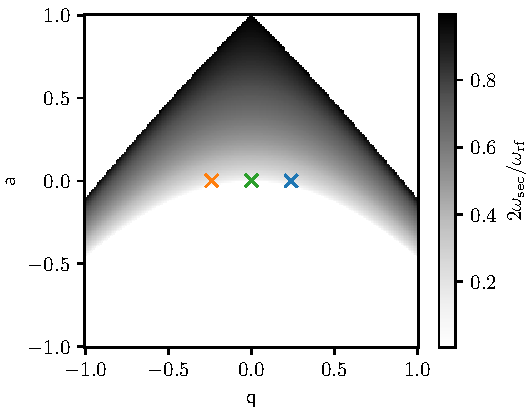
\includegraphics[width=\linewidth]{graphics/pure-mathieu-stability--presentation.pdf}
    \caption{\textit{Mathieu Stability Diagram}}
\end{figure}
\end{column}

\end{columns}    
\end{frame}

\begin{frame}{Simulation's Initial Conditions}

Important for thermal equilibrium at $t=0$:
\begin{itemize}
    \item Avoid \emph{sloshing} (center of mass movement)
    \item Avoid ion cloud \emph{breathing}
\end{itemize}

$$\mathcal{P}(v_i ;m) = \sqrt{\frac{m}{2\pi K_\mathrm{B}T}} \exp\left(-\frac{m v_i^2}{2K_\mathrm{B} T}\right)\mathrm{d}v_i$$

Analogically:

$$\mathcal{P}(x_i ;m) = \sqrt{\frac{m \omega_\mathrm{sec(i)}^2}{2\pi K_\mathrm{B}T}} \exp\left(
  -\frac{m \omega_\mathrm{sec(i)}^2 x_i^2}{2K_\mathrm{B} T}
\right)\mathrm{d}x_i$$

\vspace{2em}

If \ce{Yb^+} has $\vec{\omega}_\mathrm{sec}$, what is $\vec{\omega}_\mathrm{sec}'$ of \ce{CHDBrI^+}?

\end{frame}

\begin{frame}{Deviations from a Harmonic Trap}
\begin{columns}

\begin{column}{0.46\textwidth}

$$ \omega_\mathrm{sec(target)} \neq \omega_\mathrm{sec(cooler)}\sqrt{\frac{m_\mathrm{cooler}}{m_\mathrm{target}}} $$

Because:
$$(\tilde{a},\tilde{q}) \propto \frac{1}{m_\mathrm{cooler}}$$

So:
$$\omega_\mathrm{sec(target)} \leftarrow (\tilde{a},\tilde{q})\cdot\frac{m_\mathrm{cooler}}{m_\mathrm{target}}$$

\end{column}

\begin{column}{0.54\textwidth}
\begin{figure}
    \centering
    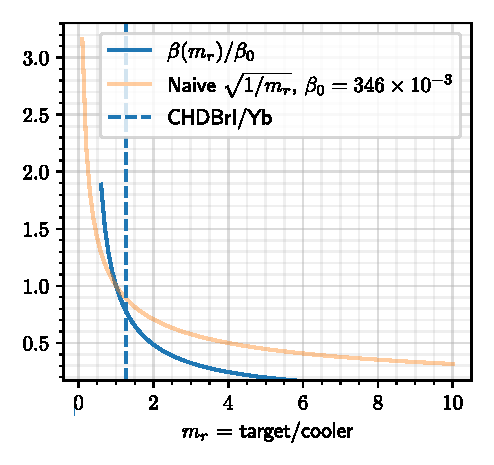
\includegraphics[width=\linewidth]{graphics/mathieu-mass-dep--presentation.pdf}
\end{figure}
\end{column}

\end{columns}
\end{frame}

\begin{frame}{Laser Cooling Model}

\begin{equation*}
    \boxed{\left\langle\mathbf{F}_\mathrm{rad}\right\rangle(\mathbf{v}; \mathbf{k}; \delta, \Omega) =  \frac{h \Gamma \hat{k}}{2\lambda} \cdot \frac{\Omega^2/2}{\Gamma^2/4 + \Omega^2/2 + (\delta -\mathbf{k}\cdot\mathbf{v})^2}}
\end{equation*}

Parameters:
\begin{itemize}
    \item \textbf{$\boldsymbol{\delta}$ - laser detuning}
    \item $\Omega$ - Laser Rabi frequency ($\propto \sqrt{I}$)
    \item $\Gamma$ - Transition level's linewidth
\end{itemize}

\end{frame}

\begin{frame}{Laser Cooling Force Offset}
\begin{columns}

\begin{column}{0.5\textwidth}
\begin{figure}
    \centering
    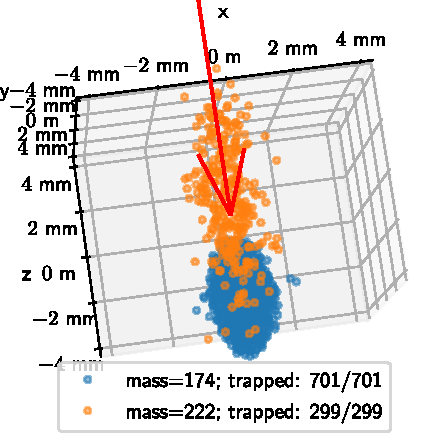
\includegraphics[width=\linewidth]{graphics/laser-cool-offset3D.pdf}
\end{figure}
\end{column}

\begin{column}{0.5\textwidth}
\begin{figure}
\centering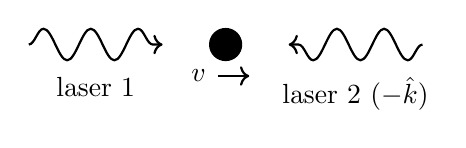
\begin{tikzpicture}
  % Left laser (Laser 1)
  \draw[->,decorate,decoration={snake,amplitude=2mm,segment length=6mm},thick] 
    (-2.5,0) -- (-0.8,0) node[midway, below=8pt] {laser 1};
  % Right laser (Laser 2)
  \visible<2->{\draw[->,decorate,decoration={snake,amplitude=2mm,segment length=6mm},thick] 
    (+2.5,0) -- (+0.8,0) node[midway, below=8pt] {laser 2 $(-\hat{k})$};}
  % Particle (black circle)
  \fill (0,0) circle (6pt);
  % Particle Velocity arrow
  \draw[->,thick] (-0.1,-0.4) -- (0.3,-0.4) node[left=12pt] {$v$};
\end{tikzpicture}
\end{figure}
$$\left\langle\mathbf{F}_\mathrm{rad}\right\rangle(\mathbf{v}; \mathbf{k}) \uncover<2->{+ \left\langle\mathbf{F}_\mathrm{rad}\right\rangle(\mathbf{v}; -\mathbf{k})}$$

\end{column}

\end{columns}
\end{frame}

\section{Main Results: Optimizations}

\subsection{Choosing Laser angle(s) (only \ce{Yb^+})}

\begin{frame}{Choosing Laser Angle(s)}
\begin{table}[h]
\centering
\begin{tabular}{lllllll}
\hline
          & $z$       & $r^-$        & $r^+$         & $e^+$      & $e^-$       & $e^*$       \\
\hline
 $\theta$ & $0^\circ$ & $67.5^\circ$ & $112.5^\circ$ & $45^\circ$ & $45^\circ$  & $-45^\circ$ \\
 $\phi$   & $0^\circ$ & $0^\circ$    & $0^\circ$     & $45^\circ$ & $-45^\circ$ & $45^\circ$  \\
\hline
\end{tabular}

\end{table}

\begin{figure}
\centering
\begin{subfigure}{0.46\textwidth}
    \centering
    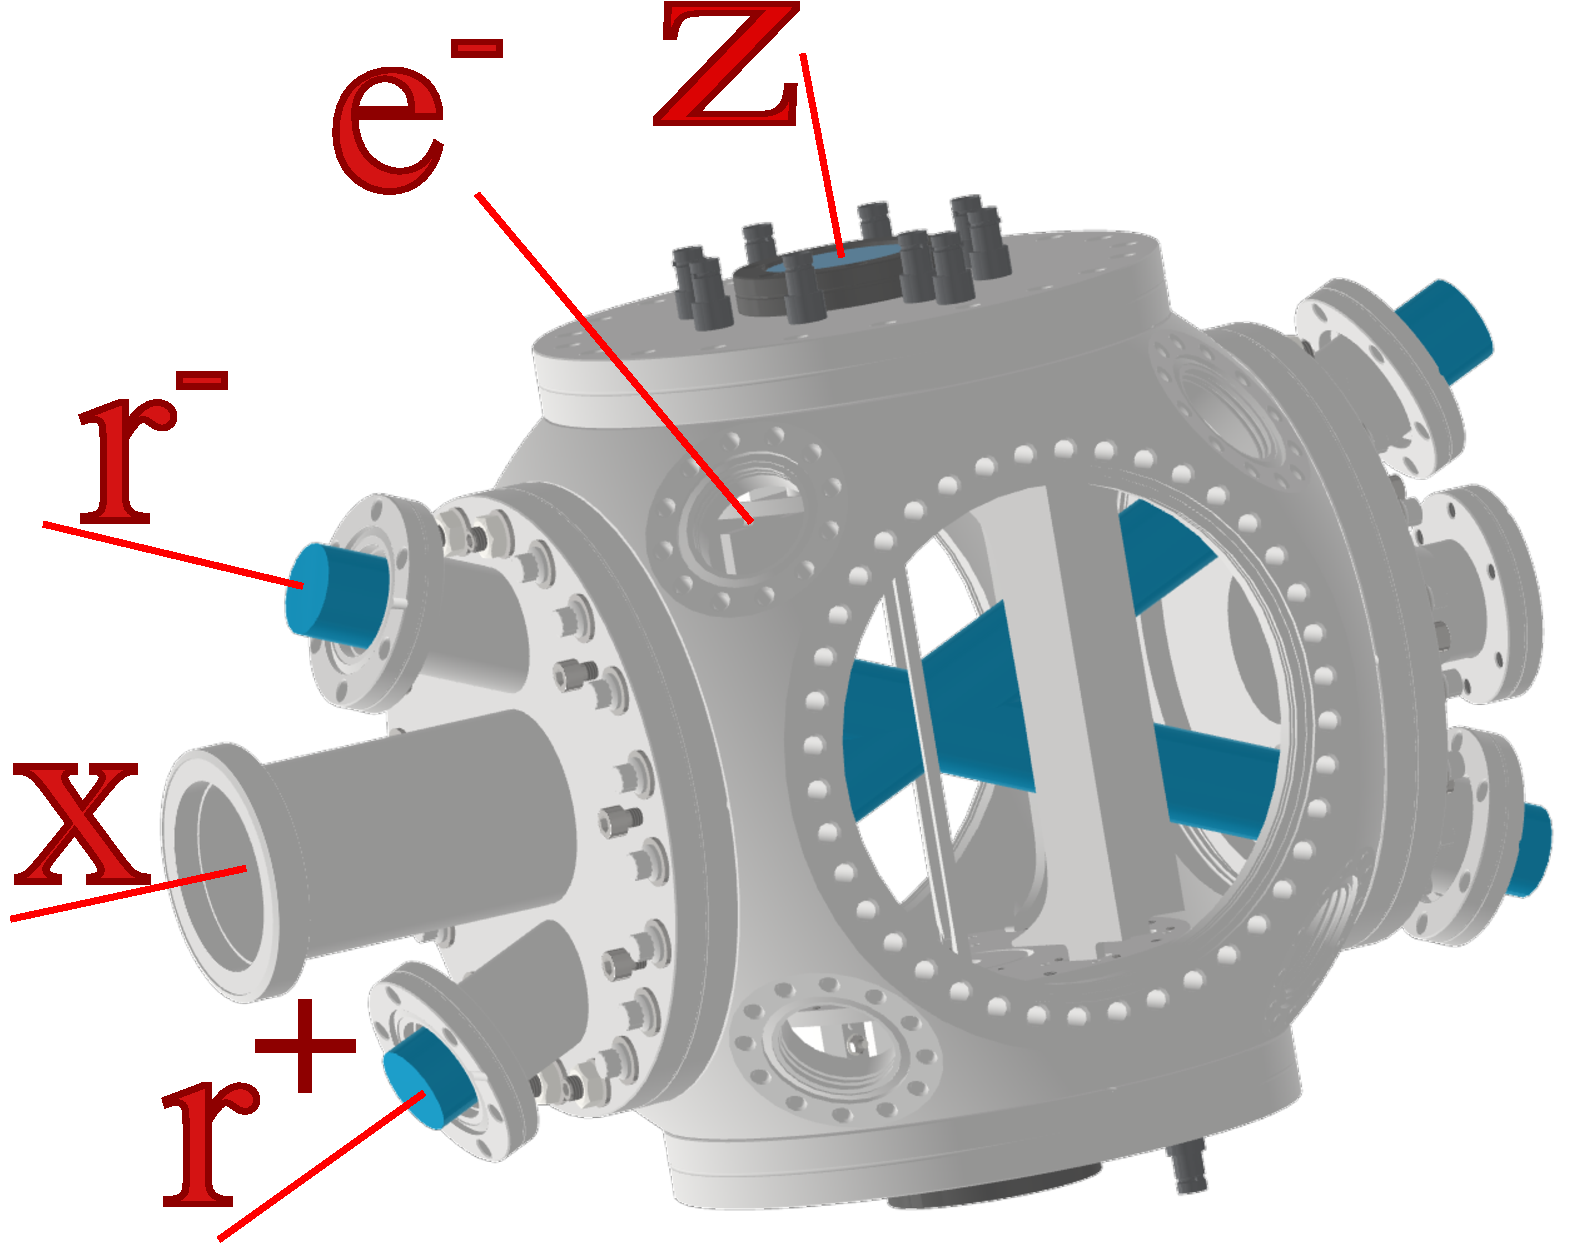
\includegraphics[width=\linewidth]{graphics/vacuum-chamber-windows.pdf}
\end{subfigure}
~
\begin{subfigure}{0.5\textwidth}
    \centering
    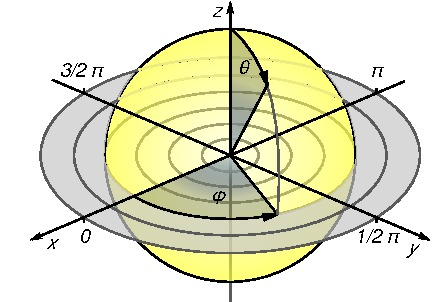
\includegraphics[width=\linewidth]{graphics/ThetaPhiAngles.pdf}
\end{subfigure}
\end{figure}
\end{frame}

\begin{frame}{Choosing Laser Angle(s)}

\begin{figure}
    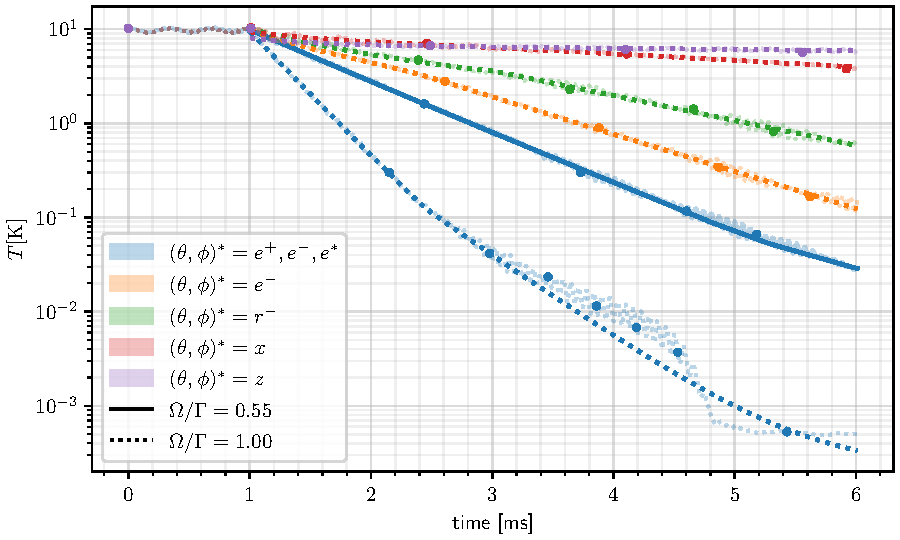
\includegraphics[width=0.9\linewidth]{graphics/laserAngles-dependence--thesis.pdf}
    \caption{\tiny $T(t)$ for several laser angles groups. For $e^+,e^-,e^*$, the per-laser-beam intensity $\Omega/\Gamma = 0.55$ sums up to $\Omega/\Gamma = 1$.}
\end{figure}

\vspace{-1em}

\begin{table}
    \tiny
    \begin{tabular}{ccccc}
    \hline
    $e^+, e^-, e^*$ & $e^-$ & $r^-$ & $x$ & $z$ \\
    \hline
    $1.3(0.0)\ \mathrm{kHz}$ & $980.7(28.1)\ \mathrm{Hz}$ & $806.3(8.4)\ \mathrm{Hz}$ & $348.8(8.0)\ \mathrm{Hz}$ & $353.0(22.2)\ \mathrm{Hz}$ \\
    \hline
    \end{tabular}
    \caption{\tiny Cooling rates computed with a linear fits to $\mathrm{Log}(T(t))$ lines presented in the figure above.}
\end{table}
\end{frame}

\subsection{Rogue \ce{Yb^+} due to crystallized \ce{CHDBrI^+}}

\begin{frame}{Adding \ce{CHDBrI^+} to Simulations}
% Say: By varying Omega and taking T_i = 5K, or taking T_i and any Omega, the Yb can stuck outside
\vspace{-1em}
\begin{columns}

\begin{column}{0.5\textwidth}
\begin{figure}
\centering
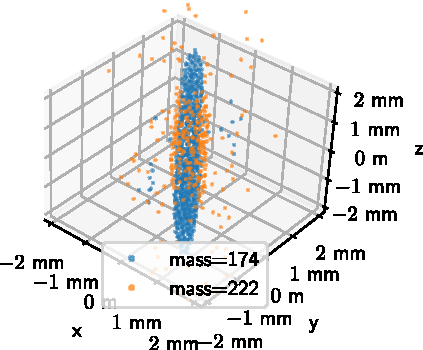
\includegraphics[width=0.8\linewidth]{graphics/Yb-Cooling-Limit/p@Ti=10O=1.pdf}
\end{figure}
\begin{figure}
\centering
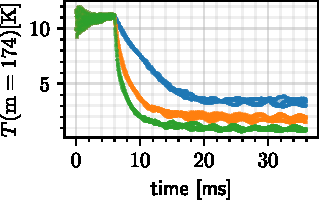
\includegraphics[width=\linewidth]{graphics/Yb-Cooling-Limit/T@Ti=10.pdf}
\end{figure}
\end{column}

\begin{column}{0.5\textwidth}

\begin{figure}
\centering
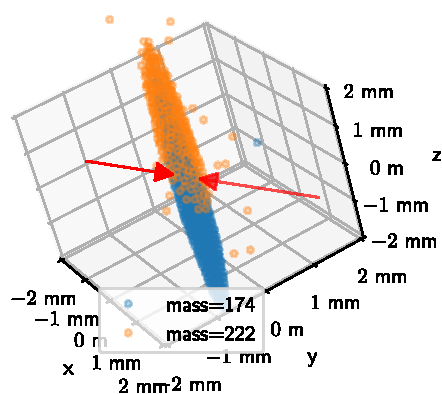
\includegraphics[width=0.8\linewidth]{graphics/Yb-Cooling-Limit/p@Ti=5O=2.5.pdf}
\end{figure}

\begin{figure}
\centering
%%%%%%%%%%%%%%%%%%%%%%%%%%%%%%%%%%%%%%%%%%%%%%%%%%%%%%%%%%%%%%%%%%
% Generated with uncommited changes! git stash diff is as follows:
%%%%%%%%%%%%%%%%%%%%%%%%%%%%%%%%%%%%%%%%%%%%%%%%%%%%%%%%%%%%%%%%%%
% diff --git a/time-plot.py b/time-plot.py
% index 890a8b6..616cf07 100755
% --- a/time-plot.py
% +++ b/time-plot.py
% @@ -138,7 +138,8 @@ class TimePlot(PlotterBase):
%                          }),
%                      )
%          self.ax.set_xlabel("time [ms]")
% -        self.ax.set_ylabel(self.ylabel)
% +        #self.ax.set_ylabel(self.ylabel)
% +        self.ax.set_ylabel("")
%          self.ax.set_yscale("log" if self.args.log else "linear")
%          if self.args.show_regimes and self.args.y == 'T':
%              averaged = self.analyzed_data.squeeze(drop=True).sel(
% 
%%%%%%%%%%%%%%%%%%%%%%%%%%%%%%%%%%%%%%%%%%%%%%%%%%%%%%%%%%%%%%%%%%
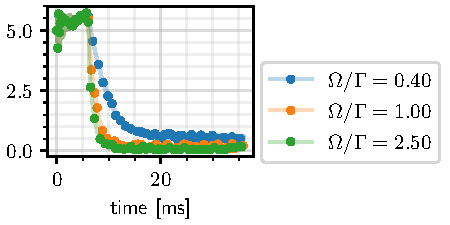
\includegraphics[width=\linewidth]{graphics/Yb-Cooling-Limit/T@Ti=5.pdf}
\end{figure}
\end{column}

\end{columns}
\end{frame}

\begin{frame}{Another Limit for \ce{CHDBrI^+}?}
Higher $\Omega$ cools fast
\begin{figure}
\centering
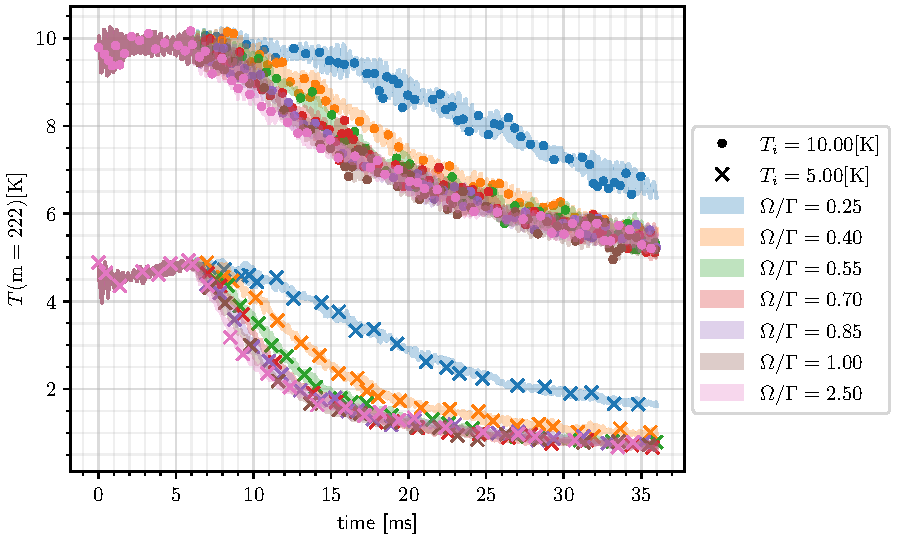
\includegraphics[width=\linewidth]{graphics/T@sympathetic-omega-dep@m=222.pdf}
\end{figure}
\end{frame}

\subsection{$T_i$ Dependence \& Angular Momentum Conservation}

\begin{frame}{$T(t)$ of \ce{CHDBrI^+} - $T_\mathrm{initial}$ Significance}{Does $T_\mathrm{CHDBrI+}$ has Memory?}
\begin{figure}
\centering
%%%%%%%%%%%%%%%%%%%%%%%%%%%%%%%%%%%%%%%%%%%%%%%%%%%%%%%%%%%%%%%%%%
% Generated with uncommited changes! git stash diff is as follows:
%%%%%%%%%%%%%%%%%%%%%%%%%%%%%%%%%%%%%%%%%%%%%%%%%%%%%%%%%%%%%%%%%%
%
% diff --git a/time-plot.py b/time-plot.py
% index a0abaaf..7c0c81e 100755
% --- a/time-plot.py
% +++ b/time-plot.py
% @@ -95,6 +95,10 @@ class TimePlot(PlotterBase):
%                      # We don't even warn here, intentionally - this is
%                      # perfectly legitimate situation.
%                      continue
% +                if label_key[0].startswith('$T_i = 5.00'):
% +                    da = da.assign_coords({
% +                        f'time|{part}': da[f'time|{part}'].values + 37.0,
% +                    })
%                  # Use .dropna to make sure the points are connected, even when
%                  # the Measurements merged had different RF divisors or
%                  # different RF frequencies, which produced an outer product of
%
%%%%%%%%%%%%%%%%%%%%%%%%%%%%%%%%%%%%%%%%%%%%%%%%%%%%%%%%%%%%%%%%%%
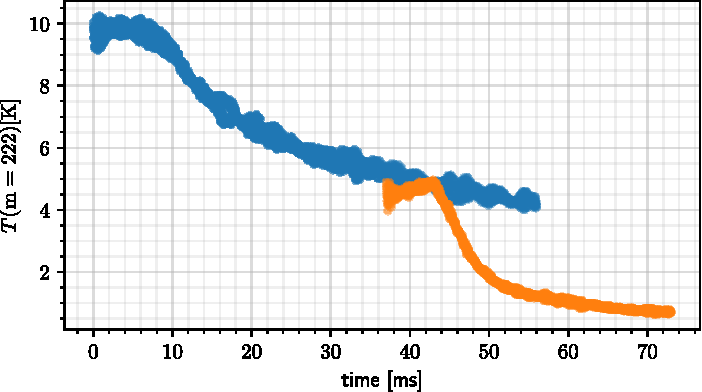
\includegraphics[width=\linewidth]{graphics/T@sympathetic-Ti-dep@m=222.pdf}
\caption{For $\Omega = 1\ \Gamma$}
\end{figure}
\end{frame}

\begin{frame}{A Sympathetic Cooling Model}
\begin{columns}

\begin{column}{0.5\textwidth}
\begin{figure}
    \centering
    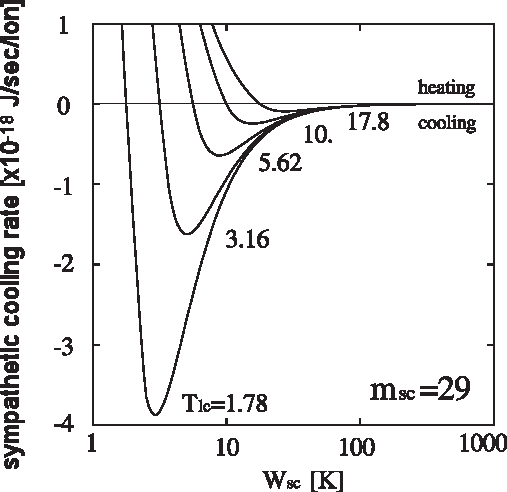
\includegraphics[width=\linewidth]{graphics/BabaWaki-CoolingRate.pdf}
    \caption{Baba \& Waki (2002), Linear traps}
\end{figure}
\end{column}

\begin{column}{0.5\textwidth}

$$T_\mathrm{sc}(t) = ?$$

Model adaptation issues:
\vspace{1em}

\centering\noindent\fbox{%
    \parbox{0.8\linewidth}{%
        All symbols are scalars!
    }%
}

\vspace{1em}
Meaning:
\vspace{1em}

\centering\noindent\fbox{%
    \parbox{0.95\linewidth}{%
        No angular momentum consideration
    }%
}

\end{column}

\end{columns}
\end{frame}

\begin{frame}{\ce{CHDBrI^+} is Rotating around $\hat{z}$ Axis!}{When Starting Hot}
\begin{columns}

\begin{column}{0.6\textwidth}
\begin{figure}
\centering
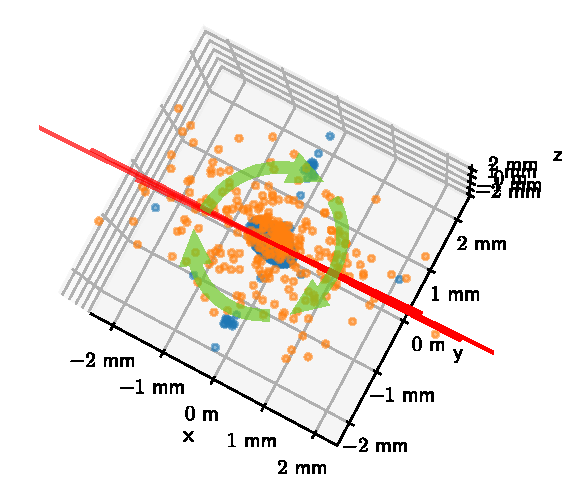
\includegraphics[width=\linewidth]{graphics/CHDBrI-Rotating-around-z.pdf}
\end{figure}
\end{column}

\begin{column}{0.4\textwidth}
\begin{figure}
    \centering
    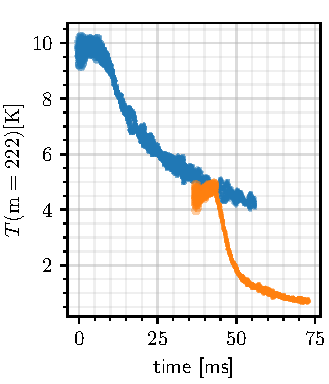
\includegraphics[width=\linewidth]{graphics/T@sympathetic-Ti-dep@m=222--narrower.pdf}
\end{figure}
\end{column}

\end{columns}
\end{frame}

\subsection{Increasing Secular Frequencies}

\begin{frame}{Another Optimization Knob: Increase $\vec{\omega}_\mathrm{sec}$}
\begin{columns}

\begin{column}{0.45\textwidth}
\begin{figure}
    \centering
    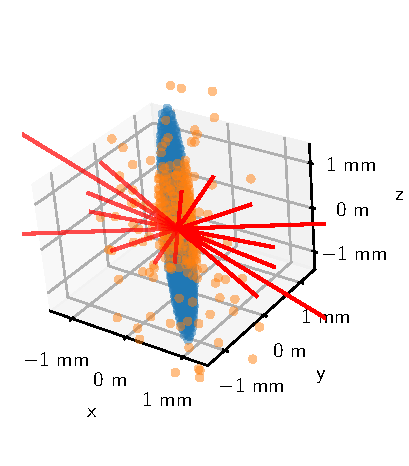
\includegraphics[width=\linewidth]{graphics/crystal-with-stronger-trap@Ti=20k.pdf}
\end{figure}
\end{column}

\begin{column}{0.55\textwidth}
\begin{figure}
\centering
\alt<2->{
    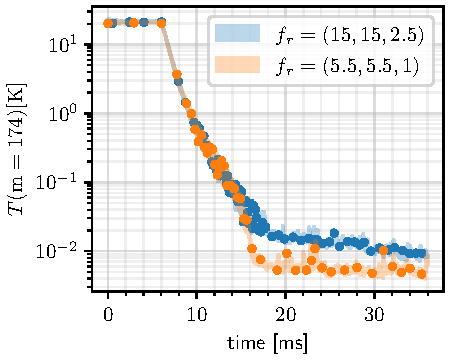
\includegraphics[width=\linewidth]{graphics/T@no-rogue-Yb.pdf}
}{
    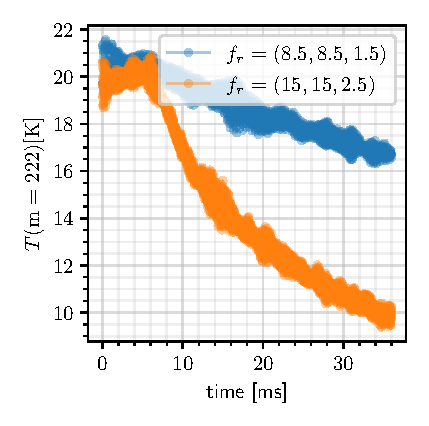
\includegraphics[width=\linewidth]{graphics/T@first-trap-comparison.pdf}
}
\caption{\alt<2->{
    \ce{Yb^+} Temperature
}{
    \ce{CHDBrI^+} Temperature (no rogue ions)
}}
\end{figure}
\end{column}

\end{columns}
\end{frame}

\begin{frame}{Scan $f_r$}
\begin{figure}
	\centering
	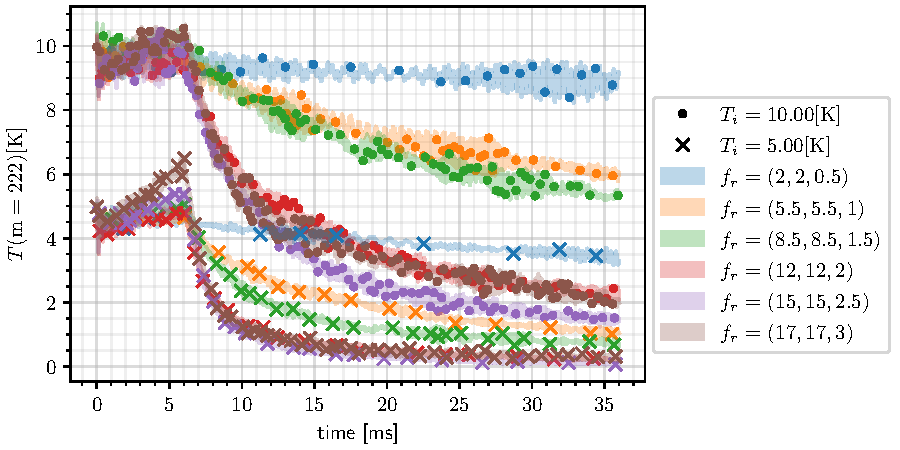
\includegraphics[width=\linewidth]{graphics/T@trap-comparison.pdf}
	\caption{Comparison of \ce{CHDBrI^+} temperatures, with $T_i \in\{5, 10\}\mathrm{K}$, and many different traps varied by color. As always, $f_r$ are in $\mathrm{kHz}$.}
\end{figure}
\end{frame}

\begin{frame}{Scan $f_r$ \& Summarize $T_f/T_i$}

\begin{figure}
\centering
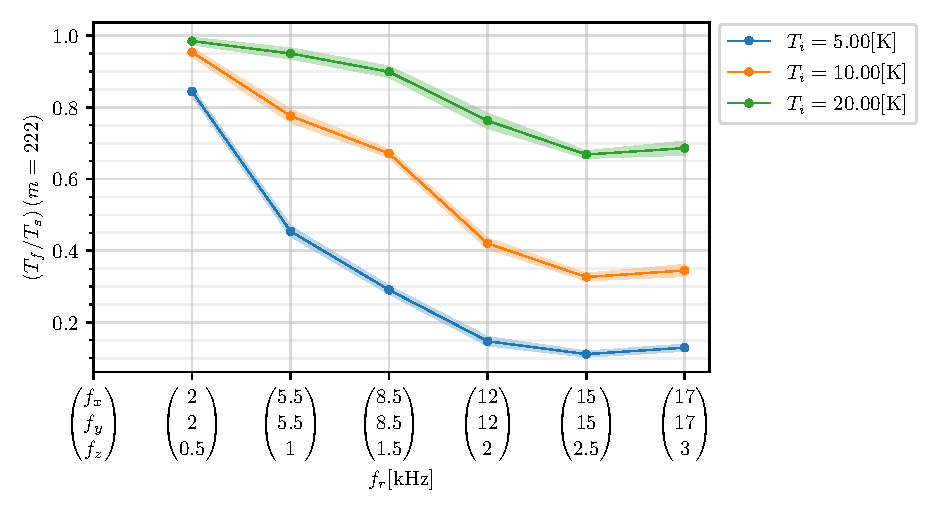
\includegraphics[width=0.98\linewidth]{graphics/trap_dependence.pdf}
\end{figure}

\vspace{-2em}

\begin{table}
	\centering
    \tiny
	\begin{tabular}{llrrl}
\hline
 $t_c \mathrm{[ms]}$   & $t_s \mathrm{[ms]}$   &   $\Omega/\Gamma$ &   $\delta/\Gamma$ & Laser's $(\theta,\phi)^*$   \\
\hline
 30.0ms                & 6.0ms                 &                 1 &              -2.6 & \begin{tabular}{lrr}
\hline
 r\^{}- &  67.5 &   0 \\
 r\^{}+ & 112.5 &   0 \\
 e\^{}- &  45   & -45 \\
\hline
\end{tabular}                             \\
\hline
\end{tabular}

\end{table}
\end{frame}

\begin{frame}{Summary}
\begin{itemize}
    \item We developed a software tool to study sympathetic cooling.
    \item Laser angles must be adjusted to trap's geometry for optimal laser cooling.
    \item Increasing $\Omega$ cools both species faster.
    \item $T_\mathrm{initial}$ is very significant for fully cooling \ce{CHDBrI^+} due to angular momentum conservation.
    \item Increasing trap's secular frequencies helps sympathetic cooling.
\end{itemize}    
\end{frame}

\section{Outlook \& Summary}

\begin{frame}{Outlook}
\begin{itemize}
    \item Simulate \& Implement a trap with:
\end{itemize}

\begin{figure}
\centering
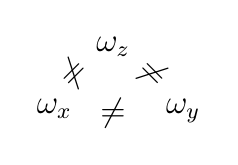
\begin{tikzpicture}[every node/.style={font=\large}]
\coordinate (A) at (0,0);
\coordinate (B) at (2,0);
\coordinate (C) at (1,1);
\node[below left]  at (0.6, 0.3) {$\omega_x$};
\node[below right] at (1.55, 0.3) {$\omega_y$};
\node[above]       at (1, 0.6) {$\omega_z$};
\path (A) -- (B) node[midway] {$\neq$};
\path (B) -- (C) node[midway, sloped] {$\neq$};
\path (C) -- (A) node[midway, sloped] {$\neq$};
\end{tikzpicture}
\end{figure}

\begin{itemize}
    \item Develop a statistical cooling model that includes angular momentum.
\end{itemize}

\begin{figure}
\centering
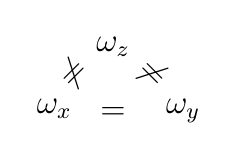
\begin{tikzpicture}[every node/.style={font=\large}]
\coordinate (A) at (0,0);
\coordinate (B) at (2,0);
\coordinate (C) at (1,1);
\node[below left]  at (0.6, 0.3) {$\omega_x$};
\node[below right] at (1.55, 0.3) {$\omega_y$};
\node[above]       at (1, 0.6) {$\omega_z$};
\path (A) -- (B) node[midway] {$=$};
\path (B) -- (C) node[midway, sloped] {$\neq$};
\path (C) -- (A) node[midway, sloped] {$\neq$};
\end{tikzpicture}
\end{figure}

\end{frame}

%%%%%%%%%%%%%%
\appendix
%%%%%%%%%%%%%

\begin{frame}{My Modeling Attempts}
\begin{columns}

\begin{column}{0.5\textwidth}

$$R_\mathrm{crystal} \approx a_\mathrm{ws} \left( N_\mathrm{lc}^{1/3} - 1.1\right)$$

\begin{figure}
    \centering
    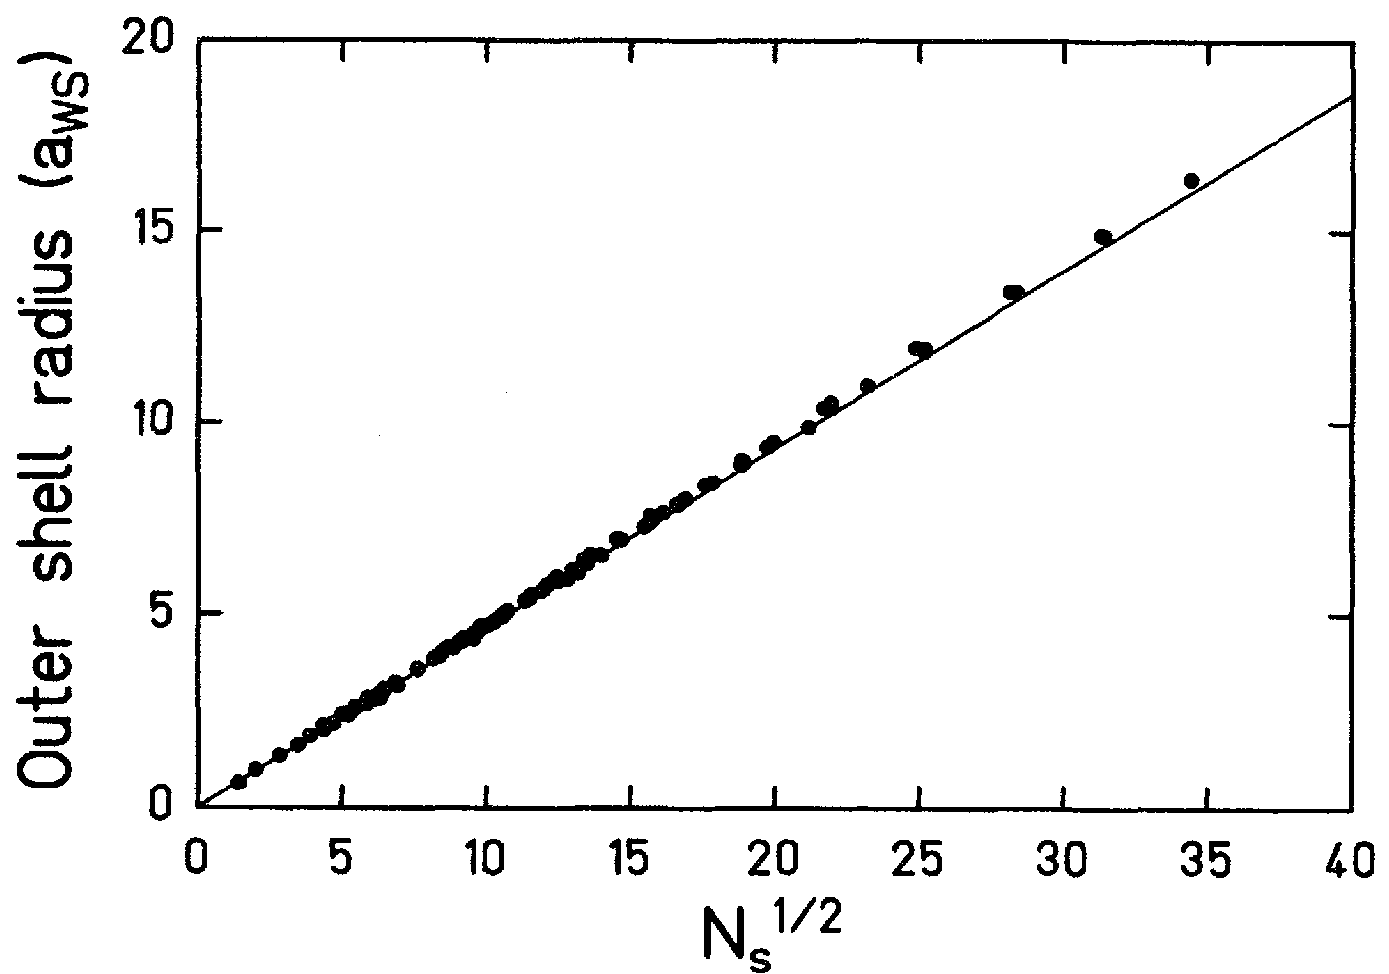
\includegraphics[width=\linewidth]{graphics/OuterShellRadius.png}
    \caption{R.W.Hasse \& V.V.Avilov (1991)}
\end{figure}
\end{column}

\begin{column}{0.5\textwidth}
$$\mathbf{a}_\mathrm{ws} = \sqrt[3]{\frac{q^2}{4\pi\varepsilon_0 m_\mathrm{lc}}}\begin{pmatrix}
    \omega_x^{-2/3} \\ \omega_y^{-2/3} \\ \omega_z^{-2/3}
\end{pmatrix}$$

$$\mathbf{R}_\mathrm{sc} \approx \sqrt{\frac{K_\mathrm{B}T_\mathrm{sc}}{m_\mathrm{sc}}}\begin{pmatrix}
    \omega_x^{-1} \\ \omega_y^{-1} \\ \omega_z^{-1}
\end{pmatrix}$$
\centering (Boltzmann)
$$\partial_t T_\mathrm{sc} \neq f(\vec{\omega}, N_\mathrm{lc}, T_\mathrm{sc})$$

\begin{itemize}
    \item Trap Symmetry?
    \item Angular Momentum?
\end{itemize}

\end{column}

\end{columns}
\end{frame}

\begin{frame}{Ideal Laser Cooling $(\Omega, \delta)$ Model}{No sympathetic cooling involved}
\begin{columns}

\begin{column}{0.5\textwidth}

\vspace{-1em}

\begin{figure}
\centering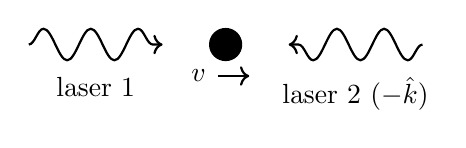
\begin{tikzpicture}
  % Left laser (Laser 1)
  \draw[->,decorate,decoration={snake,amplitude=2mm,segment length=6mm},thick] 
    (-2.5,0) -- (-0.8,0) node[midway, below=8pt] {laser 1};
  % Right laser (Laser 2)
  \draw[->,decorate,decoration={snake,amplitude=2mm,segment length=6mm},thick] 
    (+2.5,0) -- (+0.8,0) node[midway, below=8pt] {laser 2 $(-\hat{k})$};
  % Particle (black circle)
  \fill (0,0) circle (6pt);
  % Particle Velocity arrow
  \draw[->,thick] (-0.1,-0.4) -- (0.3,-0.4) node[left=12pt] {$v$};
\end{tikzpicture}
\end{figure}
$$ \mathbf{F}(\mathbf{v}) \equiv \left\langle\mathbf{F}_\mathrm{rad}\right\rangle(\mathbf{v}; \mathbf{k}) - \left\langle\mathbf{F}_\mathrm{rad}\right\rangle(-\mathbf{v}; \mathbf{k}) = $$
$$\sum_\pm \frac{h \pi \Gamma \hat{k}}{\lambda} \cdot \frac{\pm\Omega^2/2}{\Gamma^2/4 + \Omega^2/2 + (\delta \mp \mathbf{k}\cdot\mathbf{v})^2}
$$
Boltzmann: $\mathcal{P}(v) \propto \exp\left(-\frac{m v^2}{2 K_\mathrm{B}T}\right)$

\vspace{1em}
'Macroscopic Cooling Force': $$
\tilde{F}(\Omega, \delta) \overset{\mathrm{def}}{=}\int_{-\infty}^\infty\,\mathrm{d}v\exp\left(-\frac{m v^2}{2 K_\text{B} T}\right) |\mathbf{F}(v)|
$$
\end{column}

\begin{column}{0.5\textwidth}
\begin{figure}
    \centering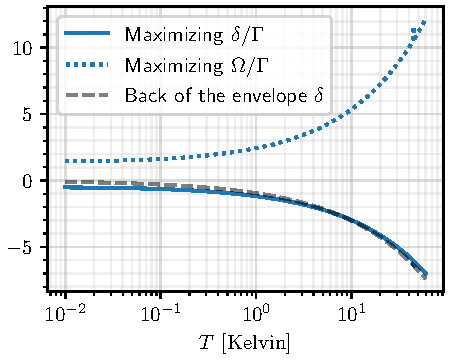
\includegraphics[width=\linewidth]{graphics/laser_cool_overlap.pdf}
\end{figure}
\centering Intuitively: $$\delta_\mathrm{opt} = \frac{\sqrt{K_\text{B} T/m}}{\lambda}$$
\end{column}

\end{columns}
\end{frame}

\begin{frame}{How Fast to Cool?}
\begin{columns}
    
\begin{column}{0.85\textwidth}

\begin{itemize}
    \item Decoherence Mechanisms:
    \begin{itemize}
        \item Room Temperature Vacuum Chamber's Black Body Radiation \& Natural vibrational level lifetime $\tau_6 = 8.79\ \mathrm{s}$
        \item Kinetic Collisions between molecular ions - Temperature
        \item Imperfect Vacuum - kinetic collisions with other particles
    \end{itemize}
    \item VMI \& Ion Trap
\end{itemize}
\begin{figure}
    \centering
    \alt<2->{
    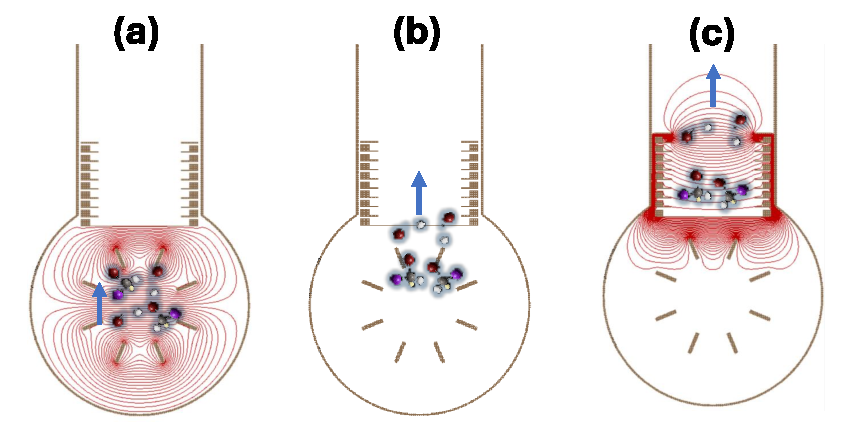
\includegraphics[width=0.9\linewidth]{graphics/trapping-and-VMI.pdf}
    }{
    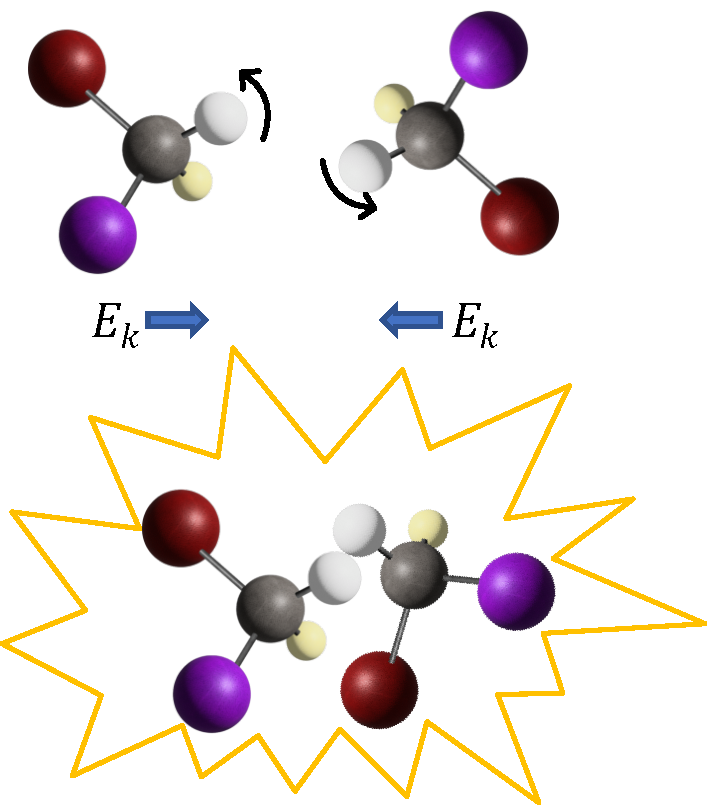
\includegraphics[width=0.35\linewidth]{graphics/Decoherence.pdf}
    }
\end{figure}
\end{column}

\begin{column}{0.18\textwidth}
\uncover<2->{\begin{figure}
    \centering
    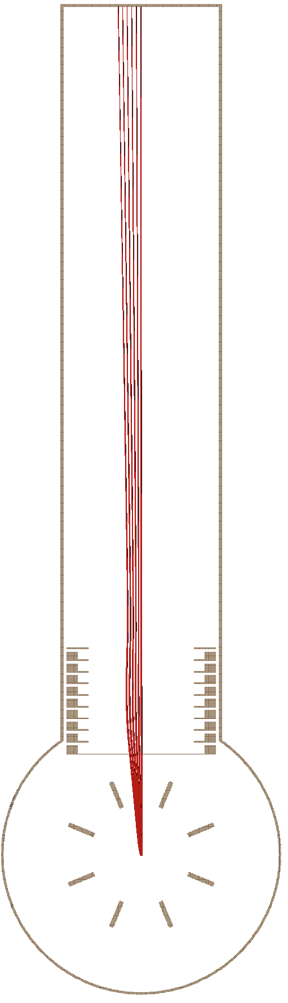
\includegraphics[width=\linewidth]{graphics/VMI-resolution.png}
\end{figure}}
\end{column}

\end{columns}
\end{frame}

\begin{frame}{Laser Cooling Model}{Bloch Equations}
\begin{equation*}
\mathcal{H}_0 = \frac{p^2}{2m} + \frac{1}{2}m\omega_0^2 x^2 = \hbar \omega_0 \left(a^\dagger a +\frac{1}{2}\right),\ \mathcal{H}_\mathrm{AF} = -\mathbf{d}\cdot\mathbf{E}
\end{equation*}
\begin{equation*}
    \mathcal{H} = \mathcal{H}_0 + \mathcal{H}_\mathrm{AF},\ \partial_t \rho = \frac{i}{\hbar}[\mathcal{H}, \rho]+ \Gamma D[a]\rho
\end{equation*}
\begin{equation*}
D[a]\rho \equiv a\rho a^\dagger - \frac{1}{2}\{a^\dagger a, \rho\}\equiv \text{Lindbland super operator}
    % Say when uncovering 5: The Lindblandian is responsible for the interaction of the atom with the vaccum - like in other open quantum systems. \gamma is the dumping due to that.
\end{equation*}
\begin{equation*}
\mathbf{F} = \partial_t \mathbf{p} = \frac{i}{\hbar}[\mathcal{H},\mathbf{p}],\ \text{RWA}\ldots\Rightarrow \left\langle\mathbf{F}_\mathrm{rad}\right\rangle = \Gamma \rho_\mathrm{ee}(t\rightarrow\infty)\hbar \mathbf{k}
\end{equation*}
\begin{equation*}
    \boxed{\left\langle\mathbf{F}_\mathrm{rad}\right\rangle(\mathbf{v}; \mathbf{k}; \delta, \Omega) =  \frac{h \Gamma \hat{k}}{2\lambda} \cdot \frac{\Omega^2/2}{\Gamma^2/4 + \Omega^2/2 + (\delta -\mathbf{k}\cdot\mathbf{v})^2}}
\end{equation*}
\tiny{Derivation from: Dan Steck - \textit{Quantum and Atom Optics}}
\end{frame}

\begin{frame}{Laser Cooling Force Imperfect Oddness}

\begin{figure}
    \centering
    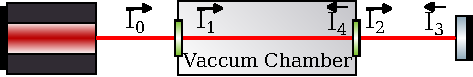
\includegraphics[width=\linewidth]{graphics/windows-attenuation.pdf}
\end{figure}

$$\frac{h\pi \Gamma\hat{k}}{\lambda} \left[\frac{\Omega^2/2}{\Gamma^2/4 + \Omega^2/2 + (\delta - \mathbf{k}\cdot\mathbf{v})^2} - \frac{\left(\alpha \Omega^2\right)/2}{\Gamma^2/4 + \left(\alpha \Omega^2\right)/2 + (\delta +\mathbf{k}\cdot\mathbf{v})^2}\right]$$

$$\text{In our system: } \alpha = \frac{I_2}{I_0} \approx 0.7$$

\end{frame}

\section{Why ions?}

\begin{frame}{In \ce{CHDBrI} \& \ce{CHDBrI^+}}
\begin{columns}

\begin{column}{0.25\textwidth}
\vspace{-2.4em}
\begin{table}[h!]
\centering
 \begin{tabular}{ll}
 \specialrule{1.8pt}{0pt}{0pt}
 1 & CBrI scissors  \\
 2 & Cl stretch \\
 3 & CBr stretch \\
 4 & CHD rock \\ 
 5 & CD wag \\
 6 & CH wag \\ 
 7 & CHD scissors \\
 8 & CD stretch \\
 9 & CH stretch \\
 \specialrule{1.8pt}{0pt}{0pt}
 \end{tabular}

\end{table}
\vspace{-1.7em}
\begin{figure}
    \centering
    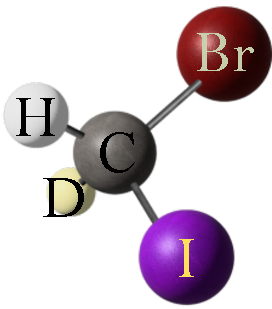
\includegraphics[width=\linewidth]{graphics/CHDBrI-labeled.pdf}
\end{figure}

\end{column}

\begin{column}{0.75\textwidth}
$\Leftarrow$ Vibrational Modes \#

\vspace{1em}

\centering Maximal $\Delta_\mathrm{PV} \approx 1.8\ \mathrm{Hz}$! ($\nu_6 \approx 33.3\ \mathrm{THz}$)

\begin{figure}
    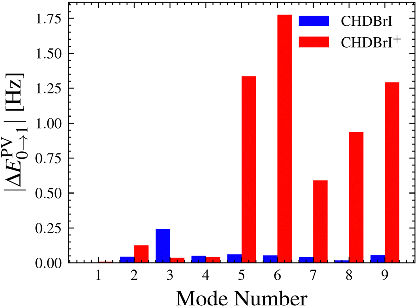
\includegraphics[width=0.8\linewidth]{graphics/CHDBrI-DeltaPV-ions-vs-neutrals.pdf}
    \caption{\small{Eduardus et al. 2023, ChemComm}}
\end{figure}
\end{column}

\end{columns}
\end{frame}

\section{Why cool? Why minimize cooling time?}

\begin{frame}{Ramsey Spectroscopy}

\begin{itemize}
    \item No need for tuning of ultra-narrow CW-IR lasers, only tuning $\delta$ - trapping duration.
    \item Directly map decoherence in time domain.
\end{itemize}

\vspace{2em}

\begin{figure}
\centering
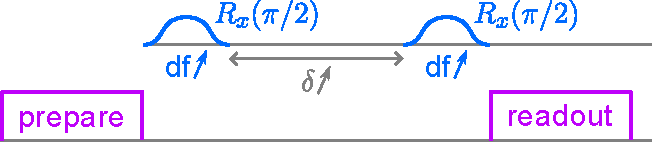
\includegraphics[width=\linewidth]{graphics/Ramsey_fringes_pulse_sequence.pdf}
\end{figure}

\end{frame}

\begin{frame}{Ramsey Spectroscopy on Molecular Ions}{Implications}
\begin{columns}

\begin{column}{0.6\textwidth}
\begin{itemize}
    \item[$+$] Trappable for long times \& can be coherent if cooled.
    \item[$-$] Can't use fluorescence for state detection due to too low ion number.
    \item[$-$] Instead, use Photo-dissociation which requires \textbf{reloading molecule for every Ramsey sequence repetition}.
\end{itemize}
\end{column}

\begin{column}{0.4\textwidth}
\begin{figure}
    \centering
    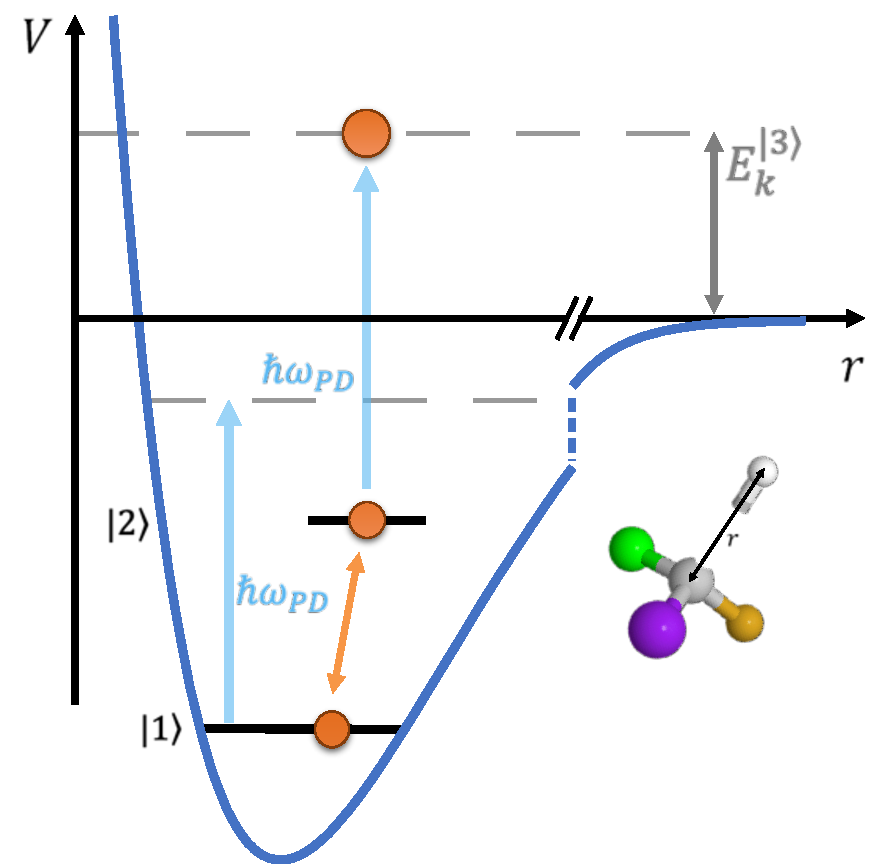
\includegraphics[width=\linewidth]{graphics/Photo-Dissociation.pdf}
\end{figure}
\end{column}

\end{columns}
\end{frame}

\begin{frame}{Ramsey Spectroscopy Statistical Uncertainty}

\begin{figure}
    \centering
    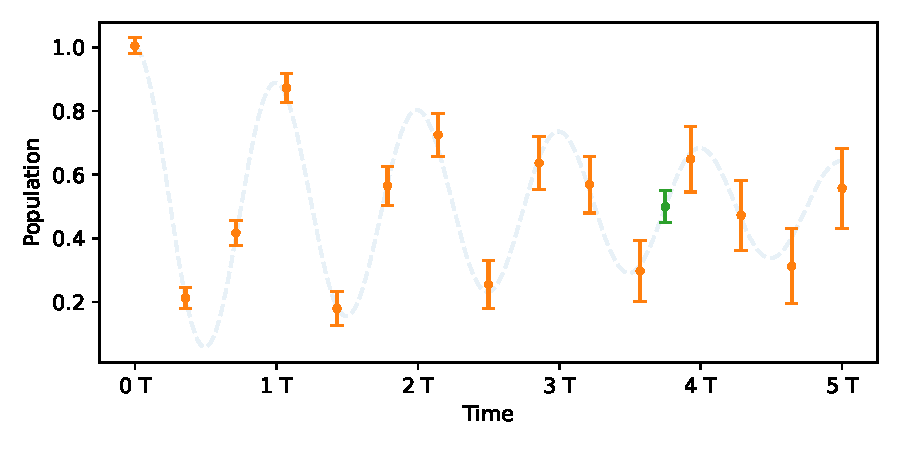
\includegraphics[width=\linewidth]{graphics/Ramsey-critical-point-marked.pdf}
\end{figure}

\vspace{-2em}
$$\frac{N}{N_0} = \frac{1}{2} \left(e^{-t/\tau} \cos(2 \pi ft + \phi) + 1\right),\ \boxed{\delta f \propto \frac{1}{\tau\sqrt{N}}}$$

\end{frame}

\begin{frame}{Cooling a Molecular Ion}{Directly? No way!}
\begin{columns}

\begin{column}{0.4\textwidth}

\begin{table}[h!]
\centering
\begin{tabular}{ll|c}
\specialrule{1.8pt}{0pt}{0pt}
\multicolumn{2}{c|}{\textbf{Mode}} & $\nu [\mathrm{cm}^{-1}]$ \\
\specialrule{1.8pt}{0pt}{0pt}
1 & CBrI scissors & 149 \\
2 & Cl stretch    & 524 \\
3 & CBr stretch   & 620 \\
4 & CHD rock      & 710 \\
5 & CD wag        & 797 \\
6 & CH wag        & 1104 \\
7 & CHD scissors  & 1275 \\
8 & CD stretch    & 2354 \\
9 & CH stretch    & 3214 \\
\specialrule{1.8pt}{0pt}{0pt}
\end{tabular}
\end{table}

\end{column}

\begin{column}{0.6\textwidth}
\begin{figure}
    \centering
    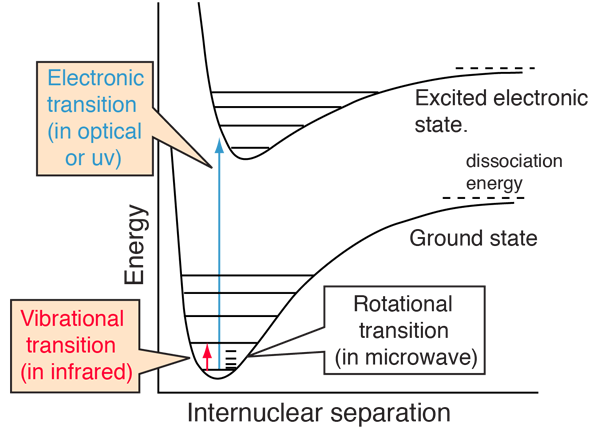
\includegraphics[width=\linewidth]{graphics/molecules-levels.png}
    \caption{Too many degrees of freedom :(}
\end{figure}
\end{column}

\end{columns}
\end{frame}

\begin{frame}{Solution: Sympathetic Cooling}
\begin{columns}

\begin{column}{0.6\textwidth}
\begin{figure}
    \centering
    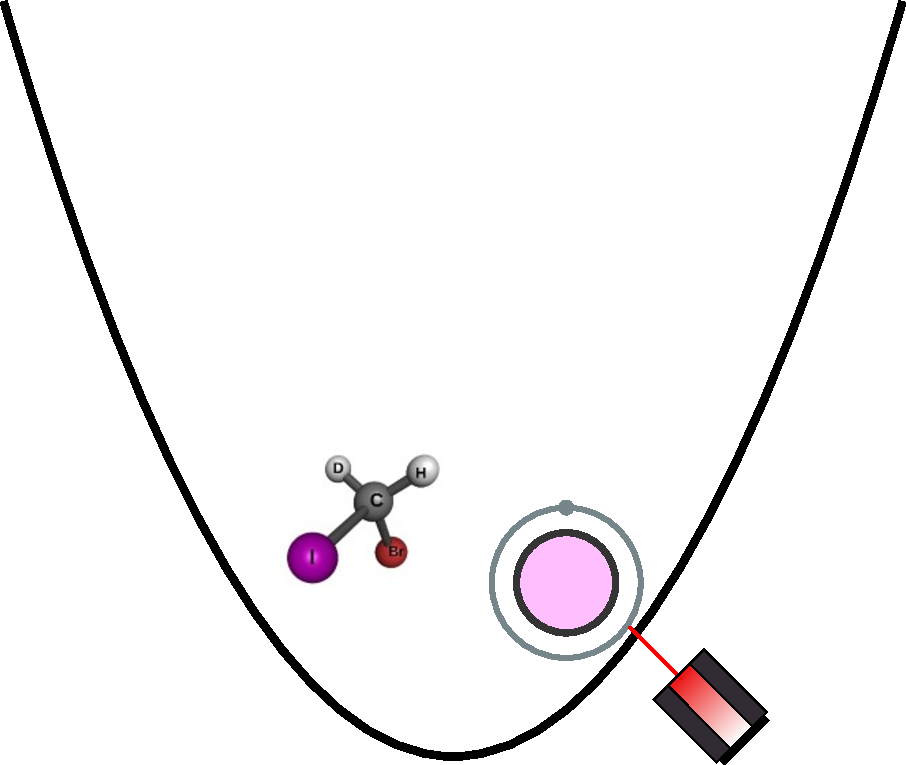
\includegraphics[width=\linewidth]{graphics/Basic-SympatheticCooling.pdf}
\end{figure}
\end{column}

\begin{column}{0.4\textwidth}
\begin{figure}
    \centering
    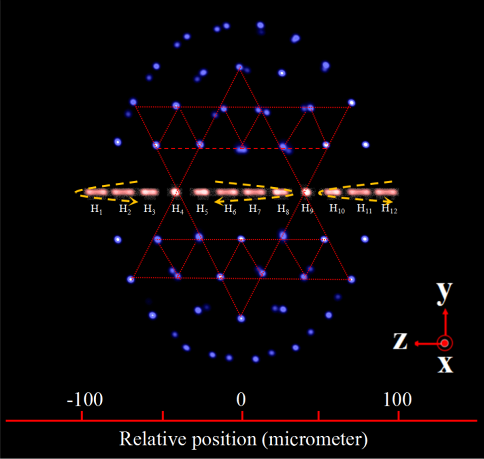
\includegraphics[width=\linewidth]{graphics/DavidStar-SC.pdf}
    \caption{Yansong Meng \& Lijun Du (2021)}
\end{figure}
\end{column}

\end{columns}
\end{frame}

\begin{frame}{What Sympathetic Cooler Species to Use?}
\begin{columns}

\begin{column}{0.7\textwidth}
\begin{figure}
    \centering
    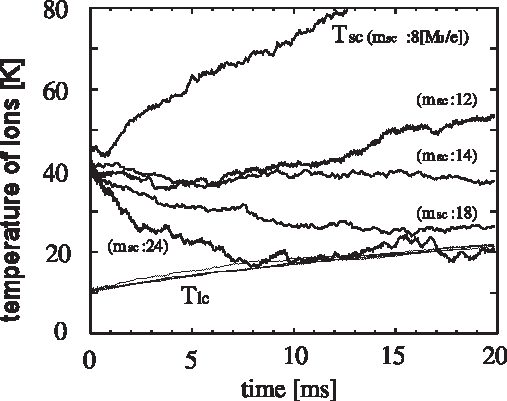
\includegraphics[width=0.8\linewidth]{graphics/Tsc-for-different-mass-ratios.pdf}
    \caption{\small{$\mathrm{sc} \equiv \text{sympathetically cooled}$, $\mathrm{lc} \equiv \text{laser cooled}$}}
\end{figure}
\vspace{-1em}
\small{From: Baba \& Waki (Japan) 2002}
\end{column}

\begin{column}{0.3\textwidth}
$$\begin{array}{lcl}
     \mathrm{sc} & \equiv & \ce{CHDBrI^+} \\
     \mathrm{lc} & \equiv & \ce{Yb^+} \\
     m_\mathrm{sc} & \approx & 222\ \mathrm{amu} \\ 
     m_\mathrm{lc} & \approx & 174\ \mathrm{amu} \\
\end{array}$$
\end{column}

\end{columns}
\end{frame}

\end{document}
